% Niveau :      PCSI *
% Discipline :  Chimie Orga
% Mots clés :   IR

\begin{exercise}{Spectre infrarouge du nitrophénol}{1}{PCSI}
{Chimie organique I,Spectroscopie,Infrarouge}{bermu}

\begin{questions}
    \question Donnez la structure de l'ortho-nitrophénol, du méta-nitrophénol et du para-nitrophénol.
    \uplevel{\paragraph{Aide :}ortho, méta et para correspondent respectivement aux positions 2, 3 et 4 sur le cycle benzénique.}

    \question Sont donnés ci-dessous les spectres IR de ces trois espèces en phase gaz. Interprétez les différences observées.
    
    \uplevel{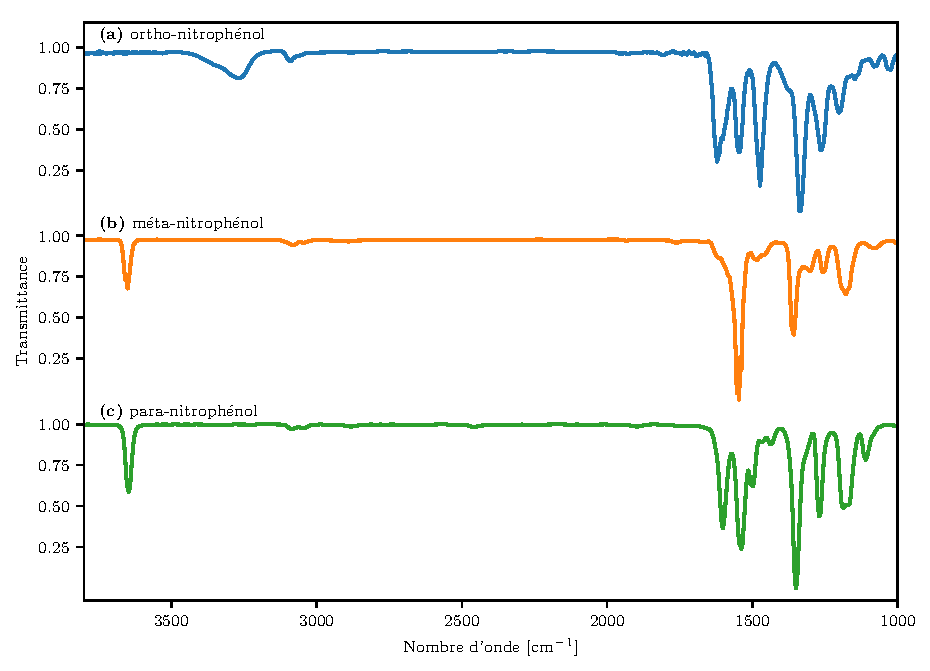
\includegraphics[width=\linewidth]{chimiePC/orga/nitro.pdf}}
    
    \question Qu'attendrait-on si les spectres étaient effectués en phase liquide ?
\end{questions}
\end{exercise}